\createTaskHeader[Zdobenie torty][9][]
Jankove narodeniny sa pomaly, ale isto blížia, a aby nebol taký smutný,
že už bude starý, Peťka mu chce upiecť jahodovú tortu. Jediné, čo sa jej
dosiaľ nepodarilo vymyslieť, je, ako tortu ozdobiť. Určite na ňu chce
zvrchu poukladať $n$ jahôd v pravidelných rozostupoch a pomedzi ne niečo
nakresliť cukrovou polevou. Zatiaľ sa s ňou ale nenaučila robiť nič iné
ako lomenú čiaru. Peťka preto chce tortu pokresliť lomenou čiarou, ktorá
pôjde od jahody k jahode, medzi dvoma jahodami vždy len rovno. Nechce
však, aby sa čiara kdekoľvek prekrížila sama so sebou, lebo by sa na tom
mieste vytvoril cukrový hrboľ, čo je veľmi neestetické. Pomôžete jej
zistiť, či sa čiara, ktorú naplánovala, prekríži?

\centerline{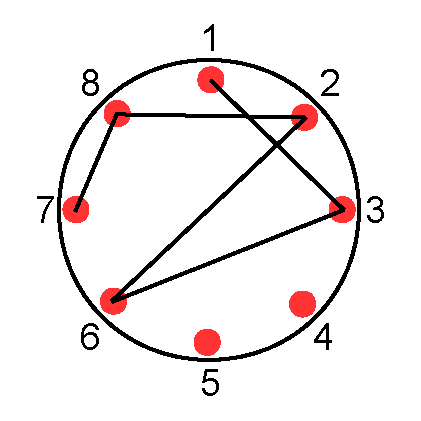
\includegraphics[height = 4cm]{sources/torta.pdf}}

\subsubsection{Úloha}

Pre zadaný kresliaci plán (čísla jahôd, medzi ktorými chce Peťka
postupne nakresliť čiaru) má váš program rozhodnúť, či sa čiara niekde
pretne sama so sebou. Je zaručené, že plán obsahuje každé číslo nanajvýš
raz.

\subsubsection{Formát vstupu}

Na prvom riadku vstupu je kladné číslo $t$ neprevyšujúce 30, určujúce
počet plánov na vstupe. Každý plán je zadaný na dvoch riadkoch, pričom
na prvom sú čísla $n, m$ ($2 \leq m \leq n \leq \num{200000}$), kde $n$
udáva počet jahôd na torte a $m$ udáva počet jahôd, medzi ktorými chce
Peťka urobiť čiaru. Na druhom riadku sú čísla $a_1, \dots, a_m$ (pričom
$1 \leq a_i \leq n$), určujúce jahody, medzi ktorými chce Peťka postupne
kresliť čiaru.

Pre polovicu vstupov platí $n = m$ (teda ak viete rozhodnúť, či sa čiara
pretne, len pre vstupy, kde čiara ide cez všetky jahody, môžete získať
polovicu bodov).

\subsubsection{Formát výstupu}

Na výstup vypíšte $t$ riadkov. Na $i$-tom má byť reťazec
``\texttt{PRETNE}'' (bez úvodzoviek) práve vtedy, keď sa čiara zadaná
$i$-tym plánom zo vstupu pretne, inak má byť na $i$-tom reťazec
``\texttt{NEPRETNE}'' (bez úvodzoviek).

\subsubsection{Príklad}

\exampleIO{
2
8 6
7 8 2 6 3 1
5 5
1 5 4 3 2
}{
PRETNE
NEPRETNE
}

\emph{V prvom prípade môžete na obrázku vidieť, že pretnutie spôsobila
posledná časť čiary od jahody 3 k jahode 1.}

\emph{V druhom prípade je jasné, že čiara sa nikde nepretne, pretože ide \uv{po obvode} -- iba
medzi susednými jahodami.}

$$\frac{\sqrt{x^3}}{c^4 \mu^3 \varepsilon_0^2} \cdot e^{i \pi} + \SI{1.34 \pm 0.7}{\kilo\gram\metre\squared\per\second\squared} \doteq
        \SI{1.4e15}{\volt\per\ampere\second}$$
    
$$\pderive[2]{\varphi}{\psi} = - \pderive[2]{\varphi}{\omega} \notin \derive{\varphi}{\theta}$$